%%% Lecture 1 Slides %%%

\documentclass{beamer}

%\documentclass[handout]{beamer}
%\usepackage{pgfpages}
%\pgfpagesuselayout{2 on 1}[a4paper,border shrink=5mm]
%\pgfpagesuselayout{1 on 1}[a4paper,border shrink=5mm]



\usepackage{amssymb}
\usepackage{amsmath}
\usepackage{mathtools}
\usepackage{tikz}
\usetikzlibrary{shapes,arrows}
\usetikzlibrary{positioning}
\usetikzlibrary{trees}
\usepackage{pgfplots}
\usepackage{pdflscape}
\usepackage{graphicx}
\usepackage{colortbl}
\usepackage{listings}
\usepackage{adjustbox}
\usepackage{physics}

\DeclarePairedDelimiter{\ceil}{\lceil}{\rceil}

\newcommand{\bs}{\boldsymbol}
\newcommand{\mb}{\mathbf}
\newcommand{\indep}{{\bot\negthickspace\negthickspace\bot}}
\newcommand{\notindep}{{\bot\negthickspace\negthickspace\bot}{\negthinspace
  \negmedspace \negthickspace \negthickspace \diagup
  \;}}
  \newcommand{\inred}[1]{\textcolor[RGB]{248,118,109}{#1}}
\newcommand{\ingreen}[1]{\textcolor[RGB]{0,191,196}{#1}}
\newcommand{\inblue}[1]{\textcolor{blue}{#1}}
\newcommand{\ind}[1]{1_{\{#1\}}}
\newcommand{\with}{\ingreen{\text{degree}}}
\newcommand{\without}{\inred{\text{no degree}}}

\renewcommand{\S}{\mb{S}}
\usepackage{color}
\definecolor{direct}{HTML}{FF0000}
\definecolor{indirect}{HTML}{FF9999}
\definecolor{dirin}{HTML}{990000}
\definecolor{control}{HTML}{999999}
\definecolor{directE}{HTML}{ED1C24}
\definecolor{indirectE}{HTML}{F69679}
\definecolor{controlE}{HTML}{999999}

%\defV{{\rm Var}\,}
\def\E{{\rm E}\,}
\def\arg{{\rm arg}\,}
\def\Cov{{\rm Cov}\,}
\def\N{{\rm N}\,}
\newcommand{\plim}{{\rm plim} \,}
\DeclareMathOperator*{\argmin}{arg\,min}
\newcommand{\X}{\mathbf{X}}
\newcommand{\Y}{\mathbf{Y}}
\newcommand{\Z}{\mathbf{Z}}
\newcommand{\I}{\mathbf{I}}
\newcommand{\V}{\mathbf{\Omega}}
\newcommand{\W}{\mathbf{W}}
\newcommand{\R}{\mathbf{R}}
\newcommand{\A}{\mathbf{A}}
\newcommand{\B}{\mathbf{B}}
\newcommand{\D}{\mathbf{D}}
\newcommand{\T}{\mathbf{T}}
\newcommand{\F}{\mathbf{F}}
\renewcommand{\O}{\mathbf{O}}
\renewcommand{\H}{\mathbf{H}}
\newcommand{\g}{\mathbf{g}}
\renewcommand{\r}{\mathbf{r}}
\newcommand{\s}{\mathbf{s}}
\newcommand{\uu}{\mathbf{u}}
\newcommand{\w}{\mathbf{w}}
\newcommand{\x}{\mathbf{x}}
\newcommand{\vv}{\mathbf{v}}
\newcommand{\z}{\mathbf{z}}
\newcommand{\y}{\mathbf{y}}

\newcommand{\bi}{\begin{itemize}}
\newcommand{\ei}{\end{itemize}}
\newcommand{\be}{\begin{enumerate}}
\newcommand{\ee}{\end{enumerate}}

\newcommand{\Beta}{\boldsymbol{\beta}}
\newcommand{\btheta}{\boldsymbol{\theta}}
\newcommand{\bgamma}{\boldsymbol{\gamma}}
\newcommand{\bpi}{\boldsymbol{\pi}}
\newcommand{\arrowp}{\stackrel{p}{\rightarrow}}
\newcommand{\arrowd}{\stackrel{d}{\rightarrow}}
\newcommand{\0}{\mathbf{0}}
\newcommand{\bP}{\mathbf{P}}
\newcommand{\nn}{\nonumber}
\def\S{{\sigma}}
\def\Supp{{\rm Supp}\,}


\newcommand\independent{\protect\mathpalette{\protect\independenT}{\perp}}
\def\independenT#1#2{\mathrel{\rlap{$#1#2$}\mkern2mu{#1#2}}}

\newcommand{\vsf}{\vspace{.5cm}}

\usepackage[english]{babel}
% or whatever

\usepackage[latin1]{inputenc}
% or whatever

\usepackage{times}
\usepackage[T1]{fontenc}
\setbeamertemplate{footline}[page number]{}
\setbeamertemplate{navigation symbols}{}


\title[Lecture 5: Inference for Subpopulation Means and Differences] % (optional, use only with long paper titles)
{Lecture 5: Inference for Subpopulation Means and Differences}


\begin{document}

\begin{frame}
  \titlepage
\end{frame}


\frame{
\frametitle{Review}

\begin{itemize}
\item In the previous lecture, we discussed learning about subpopulation proportions and differences in subpopulation proportions based on a random sample (with replacement) from the population. \pause
\item We saw that our sample subpopulation proportion was likely to be somewhat close to the subpopulation proportion (less close due to lower sample size). \pause
\item But we also demonstrated that we could accurately predict how close we might by using confidence intervals. \pause
\item We also saw that our sample difference in subpopulation proportions was likely to be somewhat close to the population difference in subpopulation proportions. \pause
\item Again, we also demonstrated that we could predict how close we might by using confidence intervals. \pause
\item We used a bootstrapping approach to confidence intervals and showed how bootstrapping differences allowed us to generate numbers that were close to the numbers in a standard regression table.
\end{itemize}

}

\frame{
\frametitle{In this lecture}

\begin{itemize}
\item In this lecture, we discuss learning subpopulation means and differences between subpopulation means based on a random sample (with replacement) from the population. \pause
\item Returning to the CPS example, we will consider 4-year degree holder incomes and income differences between 4-year degree holders and those without a 4-year degree. \pause
\item Even when the overall sample size is fixed (2246 for our example), different random samples will produce different subgroup sample sizes, and this adds a layer of complexity.  \pause
\item This complexity will not complicate our analysis much but it does complicate the justification for the analysis.
\end{itemize}

}

\frame{
\frametitle{Subsample and subpopulation means}

- A reasonable starting point for describing income in a subsample is its mean income.\\
  - We'll think about the subsample with $X_i=x$ for some value $x$, \\
  - e.g. $X_i=1$ for people with 4-year degrees.\\
- We can think of our subsample's  mean as an estimate of the mean of the corresponding finite subpopulation.\\
%- But we'll focus on interpreting it as an estimate of the mean of the *infinite subpopulation* from which they're both drawn.
%$$
%\begin{aligned}
%\hat\mu(x) &= \frac{1}{N_x} \sum_{i=1}^n (X_i) Y_i \quad \text{ for } \quad N_x = \sum_{i=1}^n \ind{x}(X_i) && \text{subsample mean} \\
%\mu(x) &= \E[Y_i \mid X_i=x] && \text{infinite subpopulation mean} \\
%\end{aligned}
%$$
%%\ind{x}
%- The subsample mean is an *unbiased estimate* of the subpopulation mean. 
%- That means its expectation *is* the subpopulation mean: $\E\{ \hat\mu(x) \} = \mu(x)$ 
%- To warm up our calculation skills, we'll prove it.
%- We'll start by reviewing a few things from probability.
}

\frame{
\frametitle{Properties of Population Means: Conditioning}

The law of iterated expectations
$$
\E\qty{ \E\qty( Y \mid X ) } \quad \text{ for any random variables $X, Y$} 
$$
To calculate the mean of $Y$, we can average within subpopulations, then across subpopulations.

 Irrelevance of independent conditioning variables
$$ \E\qty ( Y \mid X, X' ) = \E\qty( Y \mid X ) \quad \text{ when $X'$ is independent of $X,Y$ } $$
If $X'$ is unrelated to $X$ and $Y$, holding it constant doesn't affect the relationship between them.

}





\frame{
\frametitle{Properties of Population Means: Linearity}

The linearity of expectations
$$ 
\begin{aligned}
\E\qty( a Y + b Z ) 
&= \E\qty(aY) + \E\qty(bZ) \\
&= a\E(Y) + b\E(Z)  \\
& \text{ for random variables $Y, Z$ and numbers $a,b$ }
\end{aligned}
$$
  There are two things going on here.\\

  - To average a sum of two things, we can take two averages and sum.\\
  - To average a constant times a random variable, we can multiply the random variable's average by the constant.\\
  - In other words, we can *distribute* expectations and can pull constants out of them.
}

\frame{
\frametitle{The linearity of *conditional* expectations}

$$ 
\begin{aligned}
\E\qty{ a(X) Y + b(X) Z \mid X } 
&= \E\qty{a(X)Y \mid X} + \E\qty{ b(X)Z \mid X} \\
&= a(X)\E\qty(Y \mid X) + b(X)\E\qty(Z \mid X)
\end{aligned}
$$

This is like linearity of expectations, but with a twist.\\

   - When we condition on $X$, we're working with subpopulations in which $X$ is constant.\\
   - This means we can act as if functions of $X$ *are* constants.\\
   - So we can pull them out of expectations that are conditional on $X$.
}

\frame{
\frametitle{It's important to distinguish between two things}

  1.  The *conditional expectation function* $\mu(x)=\E[Y \mid X=x]$.\\
    - $\mu$ is a function; evaluated at $x$, it's a number. It's not random.\\
    - It's the mean of the infinite subpopulation of people with $X=x$.\\
   
  2.  The conditional expectation $\mu(X)=E[Y \mid X]$.\\
    - $\mu(X)$ is the mean of a *random* subpopulation of people.\\
    - It's the conditional expectation function *evaluated at* the random variable $X$.\\
    - This is the sort of thing that shows up when we use the law of iterated expectations.\\
- Let's do an easy calculation to try to make this clear. \\
- We'll calculate the mean income in our population using the law of iterated expectations. 
}

\frame{
\frametitle{Example: Conditioning}

  - Let's think about a random person drawn from this population\\
    - $Y$ is their income \\
    - $X$ is an indicator for having a four-year degree. \\
  - Suppose the subpopulation means are 100k for people with degrees
    and 50k for people without.\\
  - And that 7/10 of our population has degrees.\\
\bigskip
  What is $\E(Y \mid X)$?



  - $\E(Y \mid X)$ is a random variable that is *either* 100k or 50k\\
    - It's 100k with probability $7/10$,   when $X=1$. \\
    - And it's 50k with probability $3/10$, when $X=0$.


\bigskip

What is $\E(Y)$?



  - It's the mean of this random variable---a number.
$$
\begin{aligned} 
E\qty{ E\qty( Y \mid X ) } 
&= E(Y \mid X=1)P(X=1) + E(Y \mid X=0)P(X=0) \\
&= 100k \cdot 7/10 + 50k \cdot 3/10 = 70k + 15k = 85k.
\end{aligned}
$$

}


\frame{
\frametitle{Income and 4-year degree from the CPS}

\begin{itemize}
\item Data on 2022 household income from the CPS for individuals in California aged 25-35
\end{itemize}
\begin{table}[h]
\begin{center}
\begin{tabular}{r|r|r}
Household & income & 4-yr degree   \\
\hline
1 & 250000 &1 \\
2 & 32086 & 0 \\
$\vdots$ & $\vdots$ & $\vdots$ \\
11 & 300640 & 1\\
$\vdots$ & $\vdots$ & $\vdots$\\
2246 & 24000 & 0\\
\hline
\end{tabular}
\end{center}
\end{table}
}

\frame{
\frametitle{CPS Scatterplot}
\center
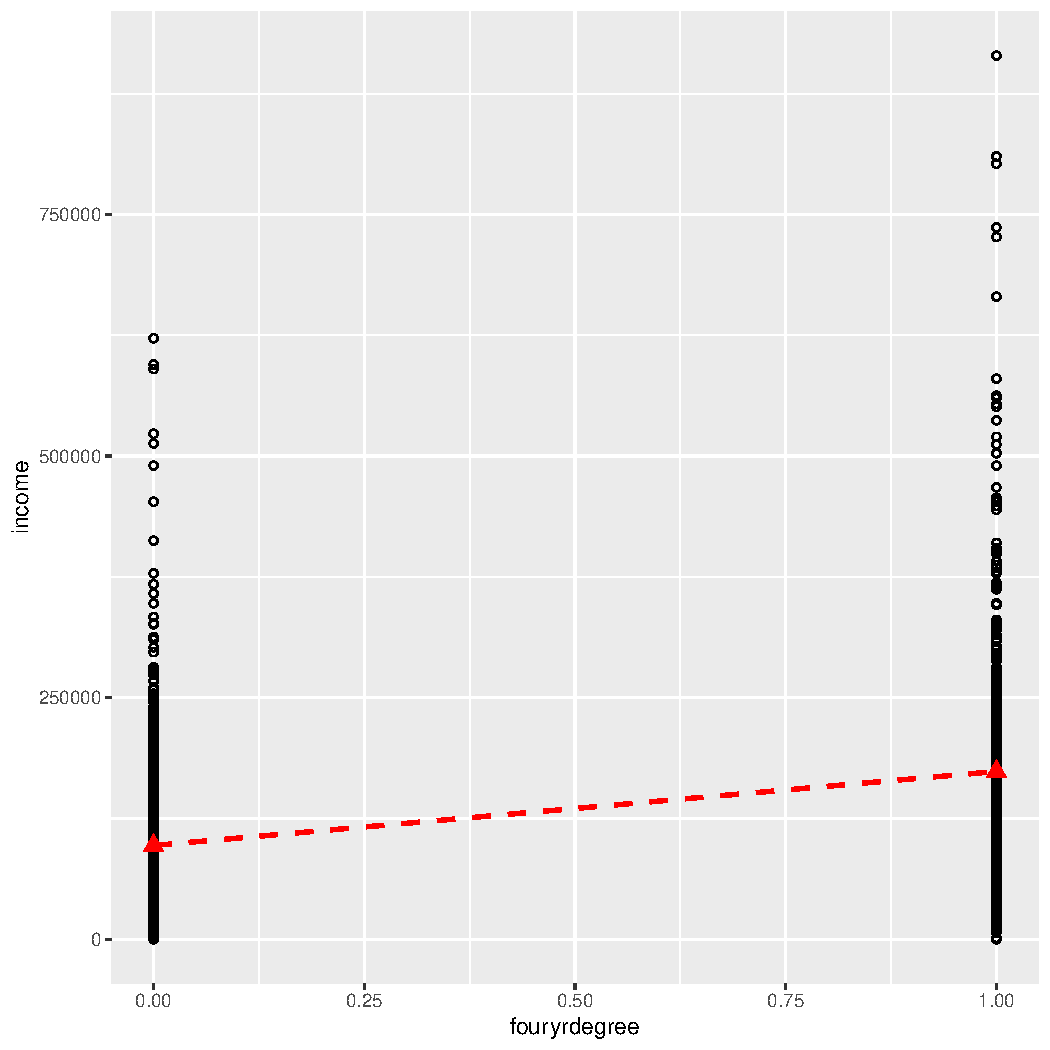
\includegraphics[scale=.45]{figs/fouryrdegree.pdf}

}



\frame{
\frametitle{CPS Sampling Distribution}

\begin{itemize}
\item Unlike the turnout example, we will never know the true subpopulation income means, which we will denote with $\mu_1$ for those with a 4-yr degree and $\mu_0$ for those without. \pause 
\item We will also never know the subpopulation income standard deviations, which we will denote $\sigma_1$ for those with a 4-yr degree and $\sigma_0$ for those without.   \pause 
\item We also will not be able to generate a sampling distribution, but we still want to know things about the sampling distribution.
\end{itemize}

}




\frame{
\frametitle{Sampling Distribution for 4-yr degree Mean Income}
\footnotesize

Let the variable $X$ take the value 1 if Black and 0 if non-Black
\begin{center}
\begin{tabular}{r|r|r|r|r|r|r}
$i$ & \multicolumn{1}{r|}{1} & \multicolumn{1}{r|}{2}   & $\dots$ & \multicolumn{1}{r|}{625} &  &  \\
\visible<1->{$s$} & $Y_1,X_1$  & $Y_2,X_2$   & $\dots$  & $Y_{2246},X_{2246}$  & $\overline{Y}_{2246}$ &  $\frac{\sum_{i=1}^{2246}Y_{i}X_{i}}{\sum_{i=1}^{2246}X_{i}} $\\
\hline
\visible<1->{1}  & 37,006,0 & 108,811,1   & $\dots$  & 49,001,0 & 129,514 & 173,671 \\
\visible<1->{2} & \visible<1->{?,?} & \visible<1->{?,?}   & \visible<1->{$\dots$}  & \visible<1->{?,?} & \visible<1->{?,?} & \visible<1->{?,?} \\
\visible<1->{3} & \visible<1->{?,?}& \visible<1->{?,?}  & \visible<1->{$\dots$} & \visible<1->{?,?} & \visible<1->{?,?} & \visible<1->{?,?} \\1-
\visible<1->{4} &  \visible<1->{?,?}& \visible<1->{?,?} & \visible<1->{$\dots$}  & \visible<1->{?,?} & \visible<1->{?,?} & \visible<1->{?,?} \\
\visible<1->{5}  & \visible<1->{?,?} & \visible<1->{?,?}  & \visible<1->{$\dots$}  & \visible<1->{?,?} & \visible<1->{?,?} & \visible<1->{?,?} \\
\visible<1->{$\vdots$}  & \visible<1->{$\vdots$} & \visible<1->{$\vdots$}   & \visible<1->{$\vdots$} & \visible<1->{$\vdots$} &  \visible<1->{$\vdots$}&  \visible<1->{$\vdots$} \\ 
\visible<1->{1 mil} & \visible<1->{?,?} & \visible<1->{?,?}& \visible<1->{$\dots$}  & \visible<1->{?,?} & \visible<1->{?,?} & \visible<1->{?,?} \\
 \visible<1->{$\vdots$}   & \visible<1->{$\vdots$} & \visible<1->{$\vdots$}  & \visible<1->{$\vdots$} & \visible<1->{$\vdots$}  & \visible<1->{$\vdots$} & \visible<1->{$\vdots$} \\ 
\hline
\visible<1->{$f_{\cdot}(\cdot)$} & \multicolumn{1}{r|}{\visible<1->{}} & \multicolumn{1}{r|}{\visible<1->{}}  &$\dots$ & \multicolumn{1}{r|}{\visible<1->{}} & \visible<1->{$N(\mu,\frac{\sigma^2}{n})$} & \visible<1->{\textcolor{red}{?}}\\
\visible<1->{$E_{\cdot}(\cdot)$} & \multicolumn{1}{r|}{\visible<1->{}} & \multicolumn{1}{r|}{\visible<1->{}}  &$\dots$ & \multicolumn{1}{r|}{\visible<1->{}} & \visible<1->{$\mu$} & \visible<1->{\textcolor{red}{?}}\\
\visible<1->{$V_{\cdot}(\cdot)$} & \multicolumn{1}{r|}{\visible<1->{}} & \multicolumn{1}{r|}{\visible<1->{}}  &$\dots$ & \multicolumn{1}{r|}{\visible<1->{}} & \visible<1->{$\frac{\sigma^2}{n}$} & \visible<1->{\textcolor{red}{?}} \\
\end{tabular}
\end{center}
\footnotesize

\begin{itemize}
\item Although we can't observe the population or the sampling distribution, we can mathematically derive certain facts about the sampling distribution. 
\item We will focus on the three red question marks.
\end{itemize}

}

\frame{


Property \#1: {\it The sampling distribution of the subsample mean is approximately normal when $\sum_{i=1}^{2246}X_{i}$ is large.}
\begin{itemize}
\item The approximate normality result comes from a central limit theorem (CLT). 
\item We know that $\frac{\sum_{i=1}^{2246}Y_{i}X_{i}}{\sum_{i=1}^{2246}X_{i}}  \sim^{approx} N(?,?)$, but still don't know the mean or the variance of this distribution. 
\end{itemize}

}

\frame{
Property \#2: {\it The subsample mean is unbiased for the subpopulation mean.} %The expected value of the sample mean,
%$\E[\frac{\sum_{i=1}^{2246}Y_{i}X_{i}}{\sum_{i=1}^{2246}X_{i}}] = \mu_1$.

\vspace{0.2in}

Part 1 of Proof (condition on $X_1=x_1, X_2=x_2,..., X_{2246}=x_{2246}$):
\begin{align*}
\E[&\frac{\sum_{i=1}^{2246}Y_{i}X_{i}}{\sum_{i=1}^{2246}X_{i}}| X_1=x_1, X_2=x_2,..., X_{2246}=x_{2246}] \\
&=\frac{1}{\sum_{i=1}^{2246}x_{i}}\E[\sum_{i=1}^{2246}Y_{i}X_{i}| X_1=x_1, X_2=x_2,..., X_{2246}=x_{2246}]  \\
&=\frac{1}{\sum_{i=1}^{2246}x_{i}} \sum_{i=1}^{2246} \E[Y_{i}X_{i}| X_1=x_1, X_2=x_2,..., X_{2246}=x_{2246}]  \\
&=\frac{1}{\sum_{i=1}^{2246}x_{i}} \sum_{i=1}^{2246} x_i\E[Y_{i}| X_1=x_1, X_2=x_2,..., X_{2246}=x_{2246}] 
\end{align*}

}


\frame{
Property \#2: {\it The subsample mean is unbiased for the subpopulation mean.} %The expected value of the sample mean,
%$\E[\frac{\sum_{i=1}^{2246}Y_{i}X_{i}}{\sum_{i=1}^{2246}X_{i}}] = \mu_1$.

\vspace{0.2in}

Part 2 of Proof (condition on $X_1=x_1, X_2=x_2,..., X_{2246}=x_{2246}$):
\begin{align*}
\frac{1}{\sum_{i=1}^{2246}x_{i}}& \sum_{i=1}^{2246} x_i\E[Y_{i}| X_1=x_1, X_2=x_2,..., X_{2246}=x_{2246}]  \\
&= \frac{1}{\sum_{i=1}^{2246}x_{i}} \sum_{i=1}^{2246} x_i\E[Y_{i}| X_i=x_i]  \\
&= \frac{1}{\sum_{i=1}^{2246}x_{i}} \sum_{i=1}^{2246} x_i[x_i\mu_1 + (1-x_i)\mu_0] \\
&=\frac{1}{\sum_{i=1}^{2246}x_{i}} \sum_{i=1}^{2246} x_i \mu_1\\
& =\frac{1}{\sum_{i=1}^{2246}x_{i}} \mu_1 \sum_{i=1}^{2246} x_i = \mu_1.
\end{align*}

}




\frame{
Property \#2: {\it The subsample mean is unbiased for the subpopulation mean.} %The expected value of the sample mean,
%$\E[\frac{\sum_{i=1}^{2246}Y_{i}X_{i}}{\sum_{i=1}^{2246}X_{i}}] = \mu_1$.

\vspace{0.2in}

Part 3 of Proof:
\begin{align*}
\E[&\frac{\sum_{i=1}^{2246}Y_{i}X_{i}}{\sum_{i=1}^{2246}X_{i}}] \\
&=\E_{\bold{X}}[\E[\frac{\sum_{i=1}^{2246}Y_{i}X_{i}}{\sum_{i=1}^{2246}X_{i}}| X_1=x_1, X_2=x_2,..., X_{2246}=x_{2246}] ]\\
&=\E_{\bold{X}}[\mu_1]\\
&=\mu_1
\end{align*}

}

\frame{
Property \#3: The {\it sampling variance} of the subsample mean,

\vspace{0.2in}

Part 1 of Proof:
\begin{align*}
V[&\frac{\sum_{i=1}^{2246}Y_{i}X_{i}}{\sum_{i=1}^{2246}X_{i}}] \\
&= \E_{\bold{X}}[V[ \frac{\sum_{i=1}^{2246}Y_{i}X_{i}}{\sum_{i=1}^{2246}X_{i}}| X_1=x_1, X_2=x_2,..., X_{2246}=x_{2246} ] ]\\
&+ V_{\bold{X}}[\E[\frac{\sum_{i=1}^{2246}Y_{i}X_{i}}{\sum_{i=1}^{2246}X_{i}}| X_1=x_1, X_2=x_2,..., X_{2246}=x_{2246} ] ] \\
&= \E_{\bold{X}}[V[ \frac{\sum_{i=1}^{2246}Y_{i}X_{i}}{\sum_{i=1}^{2246}X_{i}}| X_1=x_1, X_2=x_2,..., X_{2246}=x_{2246} ] ]\\
&+ V_{\bold{X}}[\mu_1 ]\\
\end{align*}

}

\frame{
Property \#3: The {\it sampling variance} of the subsample mean,

\vspace{0.2in}

Part 2 of Proof:
\begin{align*}
\E_{\bold{X}}[&V[ \frac{\sum_{i=1}^{2246}Y_{i}X_{i}}{\sum_{i=1}^{2246}X_{i}}| X_1=x_1, X_2=x_2,..., X_{2246}=x_{2246} ] ]\\
&= \E_{\bold{X}}[(\frac{1}{\sum_{i=1}^{2246}x_{i}})^2 V[\sum_{i=1}^{2246}Y_{i}X_{i}| X_1=x_1, X_2=x_2,..., X_{2246}=x_{2246}] ]\\
&=\E_{\bold{X}}[(\frac{1}{\sum_{i=1}^{2246}x_{i}})^2 \sum_{i=1}^{2246} V[Y_{i}X_{i}| X_1=x_1, X_2=x_2,..., X_{2246}=x_{2246}]]  \\
&=\E_{\bold{X}}[(\frac{1}{\sum_{i=1}^{2246}x_{i}})^2 \sum_{i=1}^{2246} x_i^2 V[Y_{i}| X_1=x_1, X_2=x_2,..., X_{2246}=x_{2246}]] 
\end{align*}

}


\frame{
Property \#3: The {\it sampling variance} of the subsample mean,

\vspace{0.2in}

Part 3 of Proof:
\begin{align*}
\E_{\bold{X}}[&(\frac{1}{\sum_{i=1}^{2246}x_{i}})^2 \sum_{i=1}^{2246} x_i^2 V[Y_{i}| X_1=x_1, X_2=x_2,..., X_{2246}=x_{2246}]] \\
&= \E_{\bold{X}}[(\frac{1}{\sum_{i=1}^{2246}x_{i}})^2 \sum_{i=1}^{2246} x_i^2 V[Y_{i}| X_i=x_i]] \\
&= \E_{\bold{X}}[(\frac{1}{\sum_{i=1}^{2246}x_{i}})^2 \sum_{i=1}^{2246} x_i^2 (x_i \sigma^2_1 + (1-x_i)\sigma^2_0)] \\
&= \E_{\bold{X}}[(\frac{1}{\sum_{i=1}^{2246}x_{i}})^2 \sum_{i=1}^{2246} x_i^2 \sigma^2_1] \\
&= \sigma^2_1\E_{\bold{X}}[\frac{1}{\sum_{i=1}^{2246}x_{i}}]
\end{align*}

}


\frame{
\frametitle{Sampling Distribution for 4-yr degree Mean Income}
\footnotesize

Let the variable $X$ take the value 1 if 4yr degree and 0 if not.
\begin{center}
\begin{tabular}{r|r|r|r|r|r|r}
$i$ & \multicolumn{1}{r|}{1} & \multicolumn{1}{r|}{2}   & $\dots$ & \multicolumn{1}{r|}{625} &  &  \\
\visible<1->{$s$} & $Y_1,X_1$  & $\dots$   & $\dots$  & $Y_{2246},X_{2246}$  & $\overline{Y}_{2246}$ &  $\frac{\sum_{i=1}^{2246}Y_{i}X_{i}}{\sum_{i=1}^{2246}X_{i}} $\\
\hline
\visible<1->{1}  & 37,006,0 & \dots   & $\dots$  & 49,001,0 & 135,406 & 173,671 \\
\visible<1->{2} & \visible<1->{?,?} & \visible<1->{\dots}   & \visible<1->{$\dots$}  & \visible<1->{?,?} & \visible<1->{?,?} & \visible<1->{?,?} \\
\visible<1->{3} & \visible<1->{?,?}& \visible<1->{\dots}  & \visible<1->{$\dots$} & \visible<1->{?,?} & \visible<1->{?,?} & \visible<1->{?,?} \\
\visible<1->{4} &  \visible<1->{?,?}& \visible<1->{\dots} & \visible<1->{$\dots$}  & \visible<1->{?,?} & \visible<1->{?,?} & \visible<1->{?,?} \\
\visible<1->{5}  & \visible<1->{?,?} & \visible<1->{\dots}  & \visible<1->{$\dots$}  & \visible<1->{?,?} & \visible<1->{?,?} & \visible<1->{?,?} \\
\visible<1->{$\vdots$}  & \visible<1->{$\vdots$} & \visible<1->{$\vdots$}   & \visible<1->{$\vdots$} & \visible<1->{$\vdots$} &  \visible<1->{$\vdots$}&  \visible<1->{$\vdots$} \\ 
\visible<1->{1 mil} & \visible<1->{?,?} & \visible<1->{\dots}& \visible<1->{$\dots$}  & \visible<1->{?,?} & \visible<1->{?,?} & \visible<1->{?,?} \\
 \visible<1->{$\vdots$}   & \visible<1->{$\vdots$} & \visible<1->{$\vdots$}  & \visible<1->{$\vdots$} & \visible<1->{$\vdots$}  & \visible<1->{$\vdots$} & \visible<1->{$\vdots$} \\ 
\hline
\visible<1->{$f_{\cdot}(\cdot)$} & \multicolumn{1}{r|}{\visible<1->{}} & \multicolumn{1}{r|}{\visible<1->{\dots}}  &$\dots$ & \multicolumn{1}{r|}{\visible<1->{}} & \visible<1->{$N(\mu,\frac{\sigma^2}{n})$} & \visible<1->{\textcolor{red}{$N(\mu_1, \sigma^2_1\E(\frac{1}{\sum_{i=1}^{2246}X_{i}}))$}}\\
\visible<1->{$E_{\cdot}(\cdot)$} & \multicolumn{1}{r|}{\visible<1->{}} & \multicolumn{1}{r|}{\visible<1->{\dots}}  &$\dots$ & \multicolumn{1}{r|}{\visible<1->{}} & \visible<1->{$\mu$} & \visible<1->{\textcolor{red}{$\mu_1$}}\\
\visible<1->{$V_{\cdot}(\cdot)$} & \multicolumn{1}{r|}{\visible<1->{}} & \multicolumn{1}{r|}{\visible<1->{\dots}}  &$\dots$ & \multicolumn{1}{r|}{\visible<1->{}} & \visible<1->{$\frac{\sigma^2}{n}$} & \visible<1->{\textcolor{red}{$\sigma^2_1\E(\frac{1}{\sum_{i=1}^{2246}X_{i}}))$}} \\
\end{tabular}
\end{center}
\footnotesize

\begin{itemize}
\item We still don't know $\mu_1$, $\sigma^2_1$, or $\E(\frac{1}{\sum_{i=1}^{2246}X_{i}}))$, so we have to bootstrap or estimate them.
\end{itemize}

}


\begin{frame}[fragile]
\frametitle{Simulating the Bootstrapped Sampling Distribution}


\begin{table}[h]
\begin{center}
\begin{tabular}{r|rrrr|rr}
$i$ & 1 & 2  & $\dots$ & 2,246 & $\bar{y}_{2246}$ & $\bar{y}_1 = \frac{\sum_{i=1}^{2246}y_{i}x_{i}}{\sum_{i=1}^{2246}x_{i}}$ \\
\hline
$y_i$ & 36,006 & 108,811  & $\dots$ & 49,001 & 129,514 & 173,671 \\
$x_i$ & 0 & 1  & $\dots$ & 0 & &\\
\end{tabular}
\end{center}
\end{table} 

Starting with the sample (first row of sampling distribution), each row of the bootstrapped sampling distribution is generated as the following:
\begin{verbatim}
bootind = sample(1:2246, size=2246, replace=TRUE)
dfboot = dfsam[bootind,]
subsamMean = mean(dfboot$y[dfboot$x == 1])
\end{verbatim}

\end{frame}

\begin{frame}[fragile]
\small
\begin{verbatim}
B = 10000
bootsubsamMean = rep(NA,B)
for( b in 1:B ){
bootind = sample(1:2246,size=2246,replace=T)
dfboot = dfsam[bootind,]
bootsubsamMean[b] = mean(dfboot$y[dfboot$x==1])
}
\end{verbatim}

\begin{figure}[ht] \centering
        \scalebox{.3}{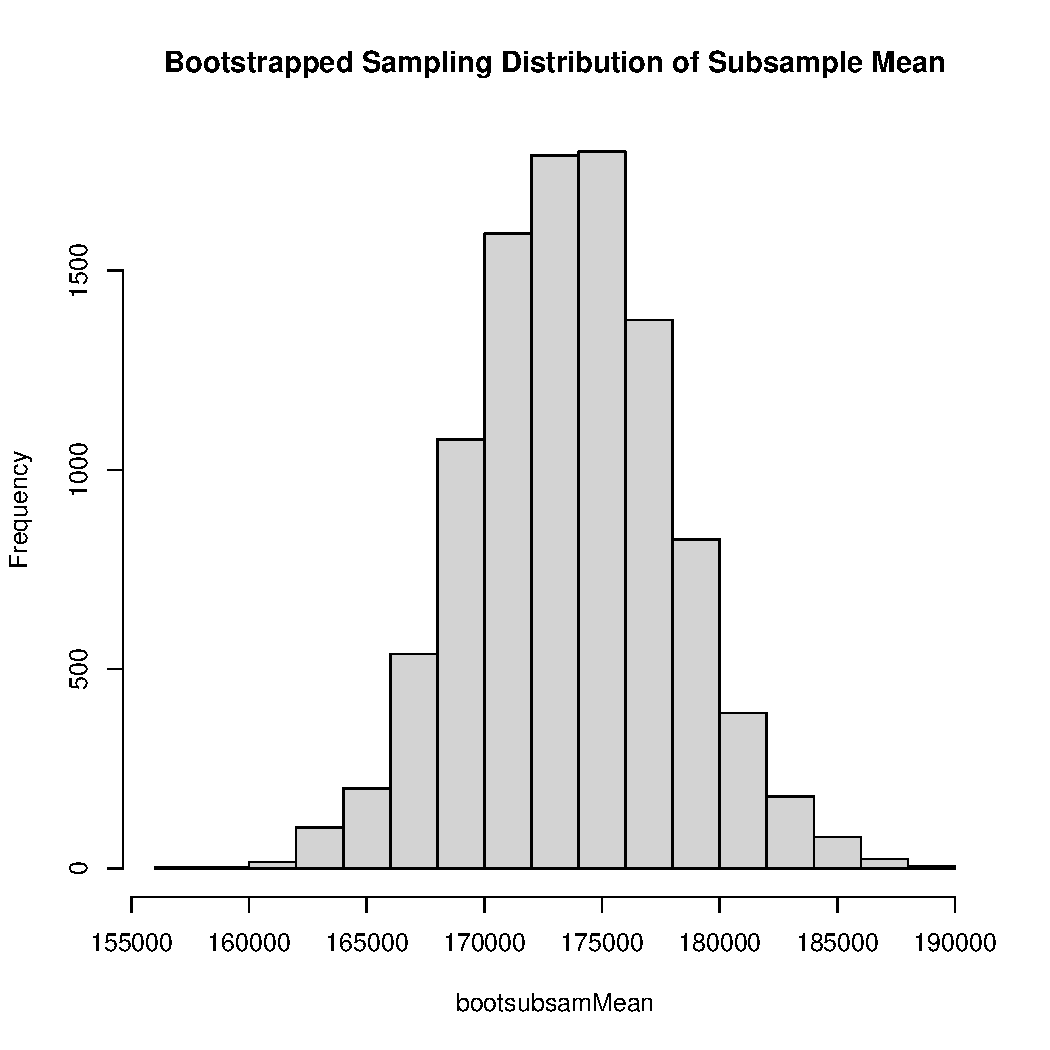
\includegraphics{figs/bootdistSub.pdf}}
\end{figure}

\end{frame}

\frame{
\frametitle{Normal Approximation CI}

Estimates
\begin{itemize}
\item $\mu_1$: $\bar y_1 = \frac{\sum_{i=1}^{2246}y_{i}x_{i}}{\sum_{i=1}^{2246}x_{i}}$
\item $\sigma^2_1$: $\frac{\sum_{i=1}^{2246}(y_{i}-\bar{y}_1)^2x_{i}}{\sum_{i=1}^{2246}x_{i}-1}$
\item $\E(\frac{1}{\sum_{i=1}^{2246}X_{i}})$: $\frac{1}{\sum_{i=1}^{2246}x_{i}}$
\end{itemize}
\bigskip
\bigskip

95\% CI:\\
$\bar y_1 \pm 1.96 \cdot \sqrt{\frac{1}{\sum_{i=1}^{2246}x_{i}} \cdot \frac{\sum_{i=1}^{2246}(y_{i}-\bar{y}_1)^2x_{i}}{\sum_{i=1}^{2246}x_{i}-1}}$

}

\frame{
\frametitle{95\% CIs}

\begin{itemize}
\item bootstrapping: [\$165,520, \$182,219]
\item approximation:  [\$165411, \$181930]
\end{itemize}
}


\section{Difference}

\frame{
\frametitle{Sampling Distribution for Difference in Mean Income}
\footnotesize

\tiny

Let the variable $X$ take the value 1 if 4yr degree and 0 if not
\begin{center}
\begin{tabular}{r|r|r|r|r|r|l}
$i$ & \multicolumn{1}{r|}{1} & \multicolumn{1}{r|}{2}   & $\dots$ & \multicolumn{1}{l|}{625} &  &  \\
\visible<1->{$s$} & $Y_1,X_1$  & $\dots$   & $\dots$  & $Y_{2246},X_{2246}$ &  $\frac{\sum_{i=1}^{2246}Y_{i}X_{i}}{\sum_{i=1}^{2246}X_{i}}$  &  $\frac{\sum_{i=1}^{2246}Y_{i}X_{i}}{\sum_{i=1}^{2246}X_{i}} - \frac{\sum_{i=1}^{2246}Y_{i}(1-X_{i})}{\sum_{i=1}^{2246}(1-X_{i})}$\\
\hline
\visible<1->{1}  & 37,006,0 & \dots   & $\dots$  & 49,001,0 & 173,671  & 76,583\\
\visible<1->{2} & \visible<1->{?,?} & \visible<1->{\dots}   & \visible<1->{$\dots$}  & \visible<1->{?,?} & \visible<1->{?,?} & \visible<1->{?,?} \\
\visible<1->{3} & \visible<1->{?,?}& \visible<1->{\dots}  & \visible<1->{$\dots$} & \visible<1->{?,?} & \visible<1->{?,?} & \visible<1->{?,?} \\
\visible<1->{4} &  \visible<1->{?,?}& \visible<1->{\dots} & \visible<1->{$\dots$}  & \visible<1->{?,?} & \visible<1->{?,?} & \visible<1->{?,?} \\
\visible<1->{5}  & \visible<1->{?,?} & \visible<1->{\dots}  & \visible<1->{$\dots$}  & \visible<1->{?,?} & \visible<1->{?,?} & \visible<1->{?,?} \\
\visible<1->{$\vdots$}  & \visible<1->{$\vdots$} & \visible<1->{$\vdots$}   & \visible<1->{$\vdots$} & \visible<1->{$\vdots$} &  \visible<1->{$\vdots$}&  \visible<1->{$\vdots$} \\ 
\visible<1->{1 mil} & \visible<1->{?,?} & \visible<1->{\dots}& \visible<1->{$\dots$}  & \visible<1->{?,?} & \visible<1->{?,?} & \visible<1->{?,?} \\
 \visible<1->{$\vdots$}   & \visible<1->{$\vdots$} & \visible<1->{$\vdots$}  & \visible<1->{$\vdots$} & \visible<1->{$\vdots$}  & \visible<1->{$\vdots$} & \visible<1->{$\vdots$} \\ 
\hline
\visible<1->{$f_{\cdot}(\cdot)$} & \multicolumn{1}{r|}{\visible<1->{}} & \multicolumn{1}{r|}{\visible<1->{\dots}}  &$\dots$ & \multicolumn{1}{r|}{\visible<1->{}} & \visible<1->{$N(\mu,\frac{\sigma^2}{n})$} & \visible<1->{\textcolor{red}{$N(\cdot, \cdot)$}}\\
\visible<1->{$E_{\cdot}(\cdot)$} & \multicolumn{1}{r|}{\visible<1->{}} & \multicolumn{1}{r|}{\visible<1->{\dots}}  &$\dots$ & \multicolumn{1}{r|}{\visible<1->{}} & \visible<1->{$\mu$} & \visible<1->{\textcolor{red}{$\mu_1-\mu_0$}}\\
\visible<1->{$V_{\cdot}(\cdot)$} & \multicolumn{1}{r|}{\visible<1->{}} & \multicolumn{1}{r|}{\visible<1->{\dots}}  &$\dots$ & \multicolumn{1}{r|}{\visible<1->{}} & \visible<1->{$\frac{\sigma^2}{n}$} & \visible<1->{\textcolor{red}{$\sigma^2_1\E(\frac{1}{\sum_{i=1}^{2246}X_{i}}) + \sigma_0^2\E(\frac{1}{\sum_{i=1}^{2246}(1-X_{i})}) $}} \\
\end{tabular}
\end{center}
\footnotesize

\begin{itemize}
\item We still don't know $\mu_1$, $\mu_0$, $\sigma^2_1$, $\sigma^2_0$, $\E(\frac{1}{\sum_{i=1}^{2246}x_{i}}))$, or $\E(\frac{1}{\sum_{i=1}^{2246}(1-x_{i})}))$, so we have to bootstrap or estimate them.
\end{itemize}

}

\begin{frame}[fragile]
\frametitle{Simulating the Bootstrapped Sampling Distribution}


\begin{table}[h]
\begin{center}
\begin{tabular}{r|rrrr|rr}
$i$ & 1 & 2  & $\dots$ & 2,246 & $\frac{\sum_{i=1}^{2246}y_{i}x_{i}}{\sum_{i=1}^{2246}x_{i}} - \frac{\sum_{i=1}^{2246}y_{i}(1-x_{i})}{\sum_{i=1}^{2246}(1-x_{i})}$ \\
\hline
$y_i$ & 36,006 & 108,811  & $\dots$ & 49,001   & 76,583 \\
$x_i$ & 0 & 1  & $\dots$ & 0 & &\\
\end{tabular}
\end{center}
\end{table} 

Starting with the sample (first row of sampling distribution), each row of the bootstrapped sampling distribution is generated as the following:
\begin{verbatim}
bootind = sample(1:2246, size=2246, replace=TRUE)
dfboot = dfsam[bootind,]
bootdiffsamMean = mean(dfboot$y[dfboot$x == 1]) - 
mean(dfboot$y[dfboot$x == 0])
\end{verbatim}

\end{frame}

\begin{frame}[fragile]
\small
\begin{verbatim}
B = 10000
bootdiffsamMean = rep(NA,B)
for( b in 1:B ){
bootind = sample(1:2246,size=2246,replace=T)
dfboot = dfsam[bootind,]
bootdiffsamMean[b] = mean(dfboot$y[dfboot$x==1]) - mean(dfboot$y[dfboot$x == 0])
}
\end{verbatim}

\begin{figure}[ht] \centering
        \scalebox{.3}{
\includegraphics{figs/bootdistDiff.pdf}}
\end{figure}

\end{frame}

\frame{
\frametitle{Normal Approximation CI}

Estimates
\begin{itemize}
\item $\mu_1-\mu_0$: $\bar y_1 -\bar y_0$
\item $\sigma^2_1$: $\frac{\sum_{i=1}^{2246}(y_{i}-\bar{y}_1)^2x_{i}}{\sum_{i=1}^{2246}x_{i}-1}$
\item $\E(\frac{1}{\sum_{i=1}^{2246}X_{i}})$: $\frac{1}{\sum_{i=1}^{2246}x_{i}}$
\item $\sigma^2_0$: $\frac{\sum_{i=1}^{2246}(y_{i}-\bar{y}_1)^2(1-x_{i})}{\sum_{i=1}^{2246}(1-x_{i})-1}$
\item $\E(\frac{1}{\sum_{i=1}^{2246}(1-X_{i})})$: $\frac{1}{\sum_{i=1}^{2246}(1-x_{i})}$
\end{itemize}
\bigskip
\bigskip

95\% CI:\\
\small
$\bar y_1 -\bar y_0 \pm 1.96 \cdot \sqrt{\frac{1}{\sum_{i=1}^{2246}x_{i}} \cdot \frac{\sum_{i=1}^{2246}(y_{i}-\bar{y}_1)^2x_{i}}{\sum_{i=1}^{2246}x_{i}-1} + \frac{1}{\sum_{i=1}^{2246}x_{i}} \cdot \frac{\sum_{i=1}^{2246}(y_{i}-\bar{y}_1)^2(1-x_{i})}{\sum_{i=1}^{2246}(1-x_{i})-1}  }$

}

\frame{
\frametitle{95\% CIs for Difference}

\begin{itemize}
\item bootstrapping: [\$67,438, \$85,865]
\item approximation:  [\$65,705, \$87459]
\end{itemize}
}




\end{document}

